\part{IHM}
\setcounter{section}{0}

\section{Enchainement des Fenêtres - EdF}

La figure suivante présente l'enchainement des fenêtres. Les quatres super-états présents dans le super état Application constituent en réalité les quatres onglets principaux de l'application. Nous avons choisi de représenter l'enchainement des fenêtres sous la forme d'un diagramme d'état qui nous permet de représenter la hierarchie en plus de la navigation contrairement à un simple diagramme de navigation dont la complexité aurait été telle qu'il aurait été illisible.

\begin{figure}[H]
\noindent\makebox[\textwidth]{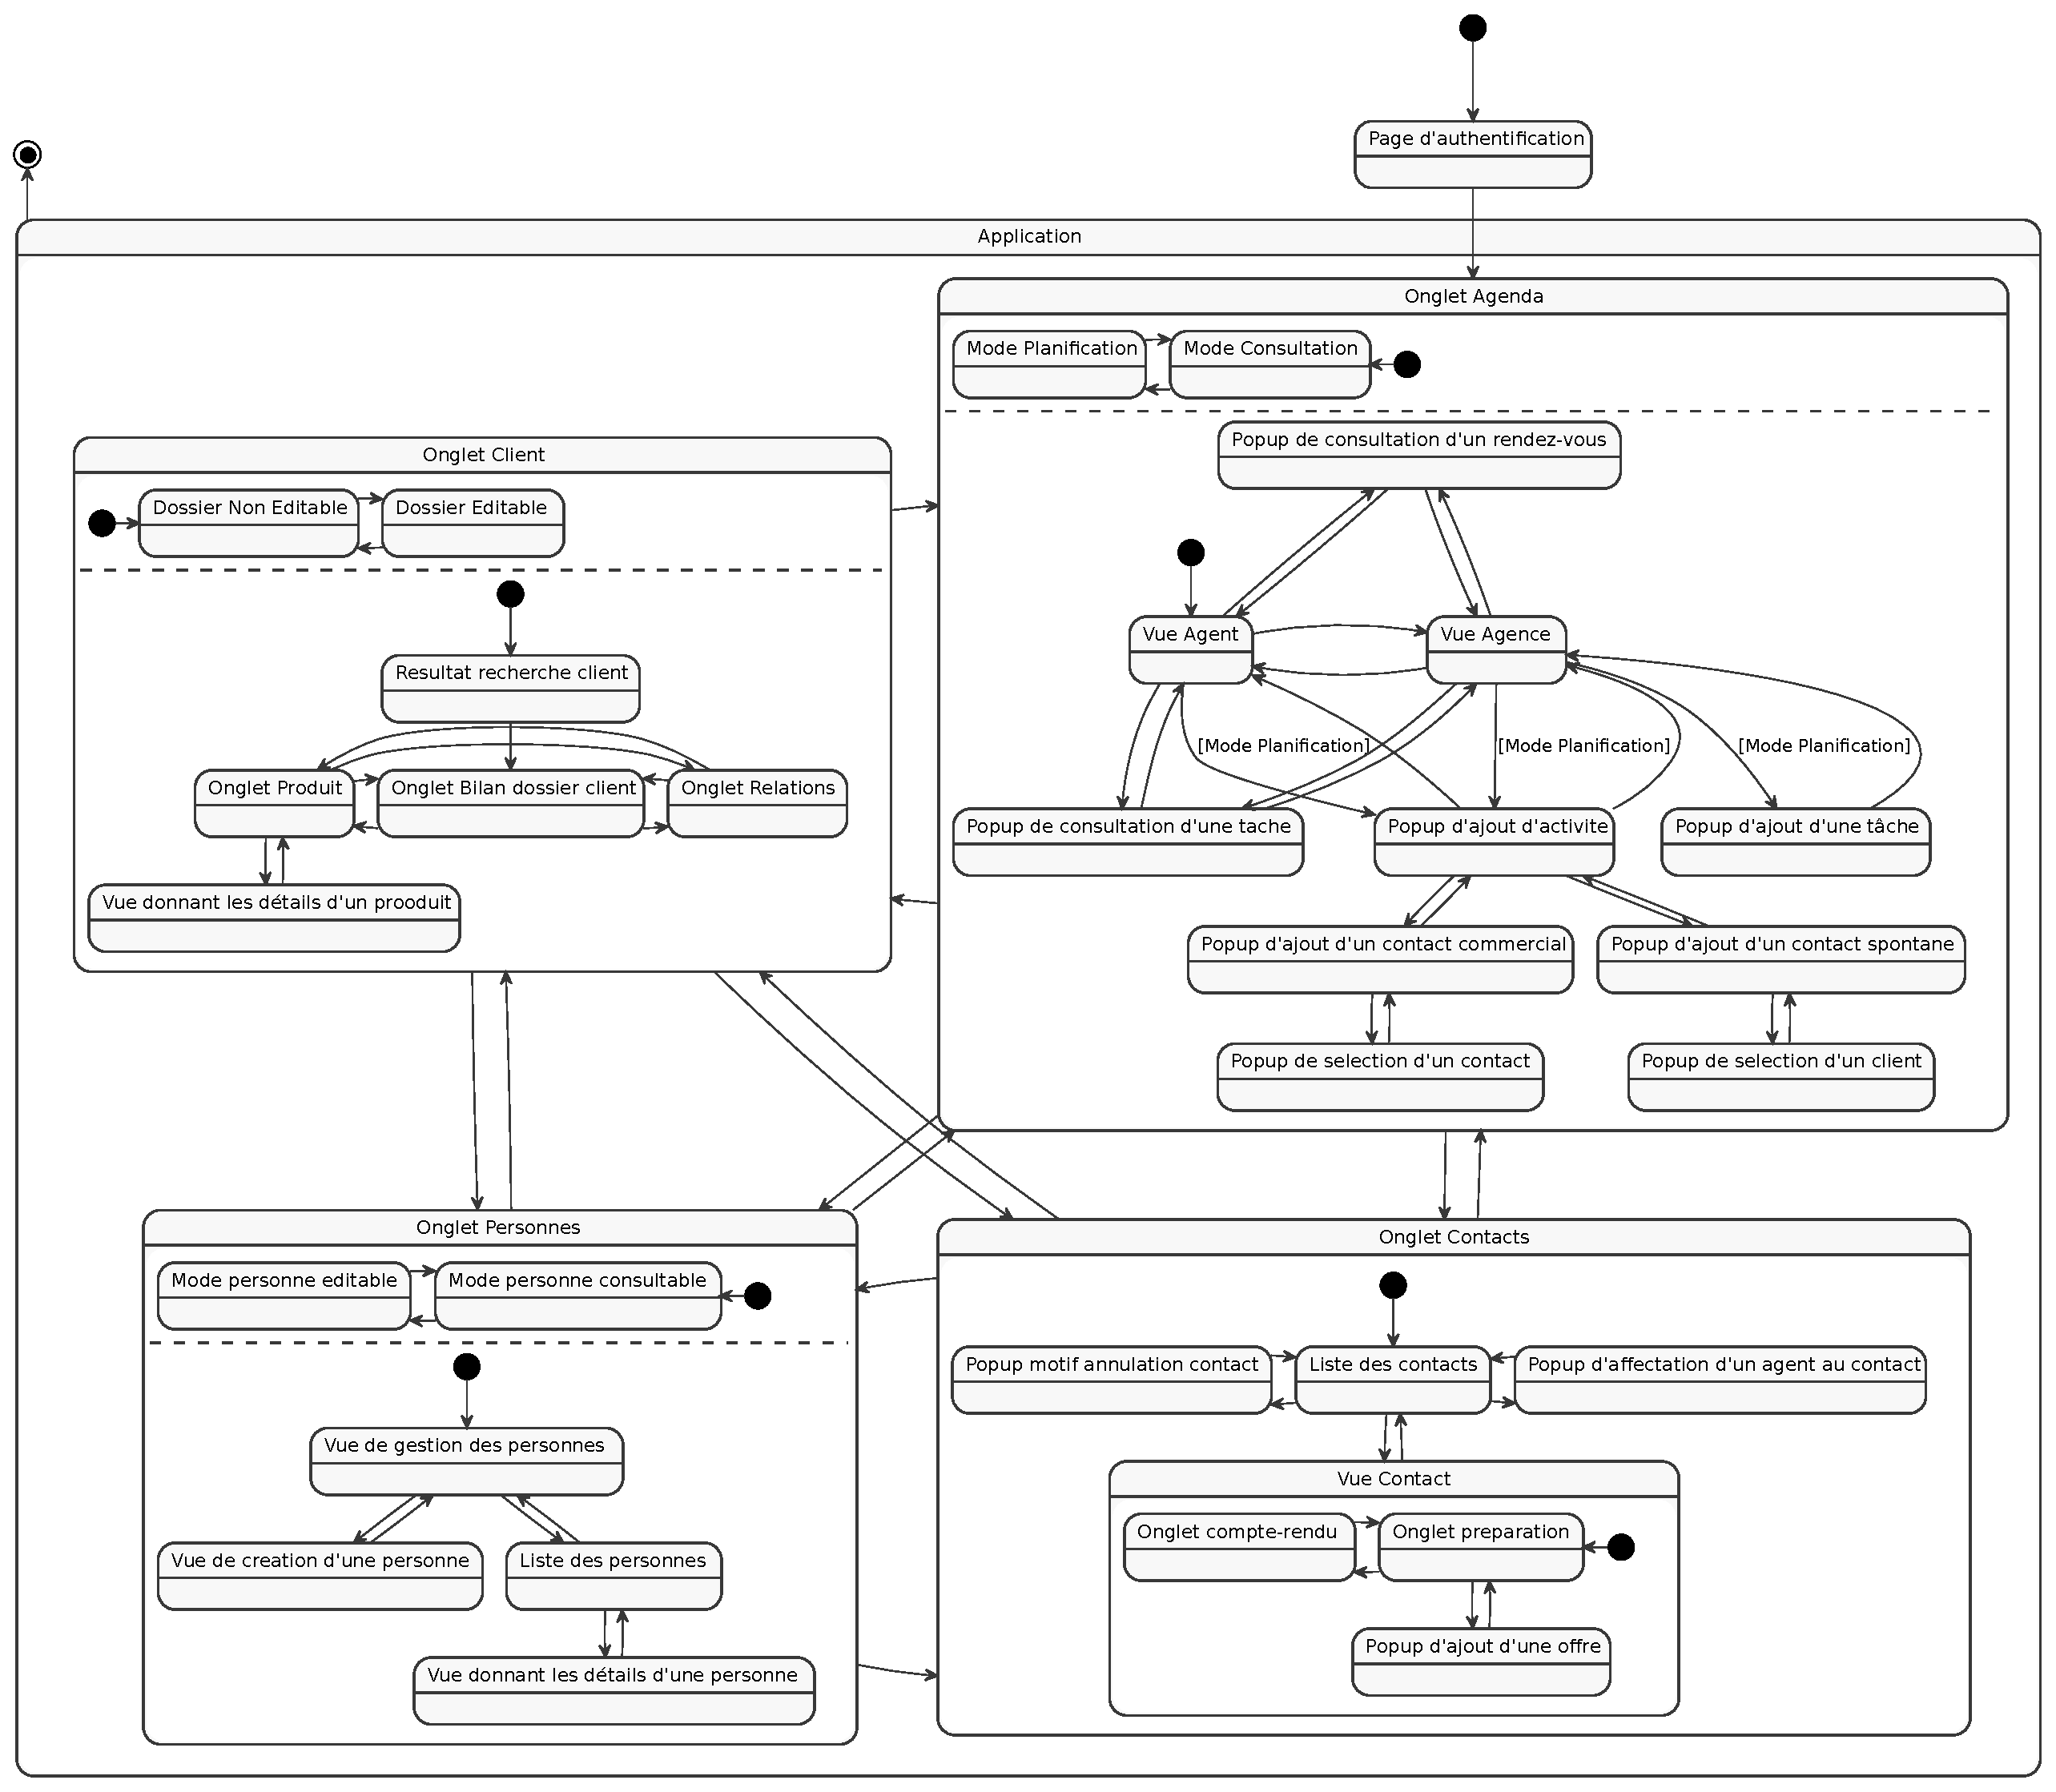
\includegraphics[width=18cm]{figures/eps/EdF}}
\caption{Diagramme d'enchainement des fenêtres}
\end{figure}

\section{Présentation des différentes vues}
Les vues de l'IHM sont présentées dans les pages suivantes.

\begin{shaded}
\textbf{Note: } Les tableaux récapitulant les SMA des différentes vues sont présentés par IHM. Si des services sont redondants, ils ont le même numéro et ne sont pas répétés dans le tableau. \\

Les cas d'utilisation des IHM sont indiqués en haut à gauche de chaque vue. La description des CU n'a pas été reportée en dessous des fenêtres. Dans le cas de manipulations qui ne sont pas immédiatement visibles, ou qui auraient engendrées une trop grosse redondance des vues, nous avons placé des commentaires sur les bords.
\end{shaded}

\begin{table}[H]
\centering
\caption{SMA - Menu}
\begin{tabular}{p{0.1\textwidth}p{0.4\textwidth}p{0.4\textwidth}}
\hline
Num & \multicolumn{1}{c}{Nom Contrôle} & \multicolumn{1}{c}{SMA} \\ \hline
\rowcolor[gray]{0.9}
\multicolumn{3}{l}{Menu}  \\
0.1 & Bouton Agenda & SM20 - ObtenirAgendaAgence \\
0.2 & Bouton Contacts & SM6 - ObtenirContactsAgent \\
\end{tabular}
\end{table}


\addcontentsline{toc}{subsection}{IHM Client}
\includepdf[scale=0.8,angle=90,pages={2-9},pagecommand=\subsection*{IHM client}]{figures/IHM.pdf}


\begin{table}[H]
\centering
\caption{SMA - IHM Client}
\begin{tabular}{p{0.1\textwidth}p{0.4\textwidth}p{0.4\textwidth}}
\hline
Num & \multicolumn{1}{c}{Nom Contrôle} & \multicolumn{1}{c}{SMA} \\ \hline
\rowcolor[gray]{0.9}
\multicolumn{3}{l}{CU10 - Recherche des clients}  \\
1.1 & Bouton Rechercher & SM46 - RechercherClient \\
\rowcolor[gray]{0.9}
\multicolumn{3}{l}{CU10 - Résultats recherche clients} \\ 
1.1 & Bouton Rechercher  & SM46 - RechercherClient       \\             
1.2 & Bouton Voir le client & SM34 - ObtenirClientEtAgence, SM35 - ConsulterBilanClient \\
\rowcolor[gray]{0.9}
\multicolumn{3}{l}{CU10 - Bilan - Dossier Client}  \\
1.3 & Bouton œil & SM36 - ConsulterDetailPersonne \\
1.4 & Bouton crayon & SM36 - ConsulterDetailPersonne \\
1.5 & Bouton poubelle & SM41 - RetirerPersonne \\
1.6 & Onglet Produits & SM43 - ObtenirProduits \\
1.7 & Onglet Relations & SM47 - ConsulterRelationsBanqueClient \\
\rowcolor[gray]{0.9}
\multicolumn{3}{l}{CU10 - Bilan - Dossier Client - Mode modification} \\ 
1.8 & Bouton Ajouter une personne  & SM39 - AjouterPersonne ou SM40 - CreerEtAjouterPersonne  \\             
1.9 & Bouton Enlever du client & SM41 - RetirerPersonne \\
1.10 & Bouton Valider & SM42 - MAJEnteteDossier \\
\rowcolor[gray]{0.9}
\multicolumn{3}{l}{CU10 - Produits - Dossier client}  \\
1.11 & Onglet Bilan & SM35 - ConsulterBilanClient \\
1.12 & Bouton Modifier (puis Valider) & SM46 - MAJComptesConcurrence \\
\rowcolor[gray]{0.9}
\multicolumn{3}{l}{CU10 - Relations - Dossier client} \\ 
1.6 & Onglet Produits & SM43 - ObtenirProduits \\
1.11 & Onglet Bilan & SM35 - ConsulterBilanClient
\end{tabular}
\end{table}

\addcontentsline{toc}{subsection}{IHM Personnes}
\includepdf[scale=0.8,angle=90,pages={10-14},pagecommand=\subsection*{IHM Personnes}]{figures/IHM.pdf}

\begin{table}[H]
\centering
\caption{SMA - IHM Personnes}
\begin{tabular}{p{0.1\textwidth}p{0.4\textwidth}p{0.4\textwidth}}
\hline
Num & \multicolumn{1}{c}{Nom Contrôle} & \multicolumn{1}{c}{SMA} \\ \hline
\rowcolor[gray]{0.9}
\multicolumn{3}{l}{CU10 - Recherche Personnes}  \\
2.1 & Bouton Rechercher & SM38 - RecupererPersonne \\
\rowcolor[gray]{0.9}
\multicolumn{3}{l}{CU10 - Resultats recherche personne}  \\
2.2 & Bouton Voir la personne & SM36 - ConsulterDetailPersonne \\
\rowcolor[gray]{0.9}
\multicolumn{3}{l}{CU10 - Detail personne}  \\
2.3 & Bouton Voir le client & SM34 - ObtenirClientEtAgence, SM35 - ConsulterBilanClient \\
\rowcolor[gray]{0.9}
\multicolumn{3}{l}{CU10 - Detail personne - Mode modification}  \\
2.3 & Bouton Voir le client & SM34 - ObtenirClientEtAgence, SM35 - ConsulterBilanClient \\
2.4 & Bouton Valider & SM37 - MettreAJourPersonne \\
\end{tabular}
\end{table}

\addcontentsline{toc}{subsection}{IHM Agenda}
\includepdf[scale=0.8,angle=90,pages={15-25},pagecommand=\subsection*{IHM Agenda}]{figures/IHM.pdf}

\begin{table}[H]
\centering
\caption{SMA - IHM Agenda}
\begin{tabular}{p{0.1\textwidth}p{0.4\textwidth}p{0.4\textwidth}}
\hline
Num & \multicolumn{1}{c}{Nom Contrôle} & \multicolumn{1}{c}{SMA} \\ \hline
\rowcolor[gray]{0.9}
\multicolumn{3}{l}{CU7 - Agenda - Agence}  \\
3.1 & Bouton Vue Agent & SM19 - ObtenirAgendaAgent \\
3.2 & Agenda - Clic sur jour & SM20 - ObtenirAgendaAgence \\
\rowcolor[gray]{0.9}
\multicolumn{3}{l}{CU7 - Agenda - Agent}  \\
3.2 & Agenda - Clic sur jour & - SM19 - ObtenirAgendaAgent \\
3.3 & Bouton Vue Agence & SM20 - ObtenirAgendaAgence \\
3.4 & ComboBox Agent & SM19 - ObtenirAgendaAgent \\
\rowcolor[gray]{0.9}
\multicolumn{3}{l}{CU7 - Agenda - Ajout contact commercial}  \\
3.5 & Bouton Ok & SM13 - EnregistrerRdv \\
3.6 & Bouton Ajouter & SM6 - ObtenirContactsAgent \\
\rowcolor[gray]{0.9}
\multicolumn{3}{l}{CU7 - Agenda - Ajout contact spontané}  \\
3.7 & Bouton Ajouter & SM48 - RechercherTousLesClients \\
3.8 & Bouton Ok & SM17 - CreerContactSpontane, SM18 - CreerRDVSpontane \\
\rowcolor[gray]{0.9}
\multicolumn{3}{l}{CU7 - Agenda - Ajout tâche}  \\
3.9 & Ajouter une activité & SM11 - CreerPlageAgenda \\
\rowcolor[gray]{0.9}
\multicolumn{3}{l}{CU7 - Agenda - clic rendez-vous}  \\
3.11 & Bouton Voir les détails & SM22 - ObtenirDetailsRdv \\
3.12 & Bouton Obtenir lettre de confirmation & SM22 - ObtenirDetailsRdv \\
3.13 & Bouton Changer la date de rendez-vous & SM23 - ModifierPlageHoraire \\
\end{tabular}
\end{table}

\addcontentsline{toc}{subsection}{IHM Contact}
\includepdf[scale=0.8,angle=90,pages={26-34},pagecommand=\subsection*{IHM Contact}]{figures/IHM.pdf}

\begin{table}[H]
\centering
\caption{SMA - IHM Contact}
\begin{tabular}{p{0.1\textwidth}p{0.4\textwidth}p{0.4\textwidth}}
\hline
Num & \multicolumn{1}{c}{Nom Contrôle} & \multicolumn{1}{c}{SMA} \\ \hline
\rowcolor[gray]{0.9}
\multicolumn{3}{l}{CU4 - Contacts - Agent}  \\
4.1 & Bouton Grouper les contacts & SM8 - GrouperContacts \\
4.2 & Combobox agents & SM6 - ObtenirContactsAgent \\
4.3 & Bouton œil & SM9 - ObtenirDetailsContact\newline SM22 - ObtenirDetailsRdv\\
\rowcolor[gray]{0.9}
\multicolumn{3}{l}{CU4 - Contacts - Agent - Annulation contact}  \\
4.4 & Bouton Supprimer & SM10 - AnnulerContact \\
\rowcolor[gray]{0.9}
\multicolumn{3}{l}{CU2 - Affectation contact}  \\
4.5 & Bouton Affecter le contact & SM5 - AffecterContact\\
\rowcolor[gray]{0.9}
\multicolumn{3}{l}{CU8 - Vue contact - Préparation d'un rendez-vous}  \\
4.6 & Bouton Voir le client & SM34 - ObtenirClientEtAgence \newline SM35 - ConsulterBilanClient \\
4.7 & Bouton Annuler rendez-vous & SM24 - AnnulerRdv\\
4.8 & Bouton Obtenir lettre de confirmation & SM22 - ObtenirDetailsRdv \\
4.9 & Combobox Agent & SM21 - ReaffecterRdv\\
4.10 & Bouton Enregistrer & SM31 - EnregistrerCompteRenduPreparation, SM30 - AnnoterProposition\\
\rowcolor[gray]{0.9}
\multicolumn{3}{l}{CU9 - Vue contact - Compte rendu entretient - Mode modification}  \\
4.11 & Bouton Enregistrer & SM33 - EnregistrerRapportActivite\\
\rowcolor[gray]{0.9}
\multicolumn{3}{l}{CU8 - Ajout d'offres}  \\
4.12 & Bouton Ajouter & SM29 - AjouterPropositionCommerciale\\
\end{tabular}
\end{table}